\section{The Razor Approach to Kinematics}
\label{sec:kinematic}

The production of supersymmetric particles at hadron colliders may be
broadly described as:
\begin{enumerate}[(i)]
\item pair production of heavy particles (such as a $\PSg$ or a
  $\PSq$), and
\item decay of the heavy particle into a set of final state
  particles consisting of a \emph{visible} subset and an
  \emph{invisible} subset (usually including the neutralino LSP $\chiz$).
\end{enumerate}
Although motivated by supersymmetry, the razor variables are intended for use in any generic new physics
scenario with visible and invisible final state particles. 

In defining the razor variables, it is useful to consider the explicit
example of squark pair production $\PSq_1\PSq_2$, where each squark
decays to a quark and a neutralino LSP $\PSq_i\to\Pq_i\chiz_{i}$, as shown in
Fig.~\ref{fig:T2}. In the following, we treat the quarks as massless.
\begin{figure*}[thb!]
\centering
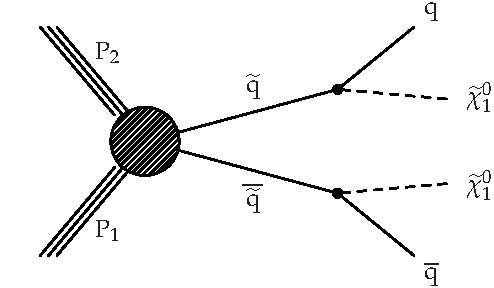
\includegraphics[width=0.49\textwidth]{figs/theory/T2.pdf}
\caption{Diagram featuring squark pair production.\label{fig:T2}}
\end{figure*}
In the the rest frame of the squarks, the momenta of the
quark and the LSP are back-to-back and satisfy 
\begin{equation}
2|\vec{p}^{\Pq_i} | = 2|\vec{p}^{\chiz_{i}} | =\sqrt{
\frac{\left[m_{\PSq}^2-(m_\cPq+m_{\chiz})^2\right]\left[m_{\PSq}^2-(m_\cPq-m_{\chiz}
    )^2\right]}{m_{\PSq}^2}} \equiv M_{\Delta} ~.
\end{equation}
% my derivation:
%\begin{equation}
% M_{\Delta} = 2\sqrt{\left(
%\frac{m_{\PSq}^2 - m_{\chiz_1}^2 + m_{\cPq}^2}{2m_{\PSq}}\right)^2 - m_{\cPq}^2}
%\end{equation}
$M_{\Delta}$ is a characteristic mass scale related to the
masses of the heavy pair-produced squark and the invisible LSP. In the
limit of massless quarks, this simplifies to 
\begin{equation}
M_{\Delta} =
\frac{m_{\PSq}^2-m_{\chiz}^2}{m_{\PSq}}~.
\end{equation}

If we could identify this rest frame, we could boost the quarks'
momenta, evaluate them in the new frame, and
gain information about the unseen sparticle masses. Unfortunately there are too many missing
degrees of freedom to do this. 

In principle, we need all eight components of the invisible particles'
four-momenta to construct the desired boosts. At a hadron collider, we only have access
only to the missing transverse momentum $\ptvecmiss$, which in the
ideal case of no initial/final state radiation (ISR/FSR), no pileup
contamination, and perfect detector measurement is $\ptvec^{\,\chiz_{1}}
+ \ptvec^{\,\chiz_{2}},$ giving us two constraints. After making the simplifying
assumption of symmetry between the two sides of the decay chain 
%(two additional constraints: $p_{\PSq_1})^2 = p_{\PSq_2})^2$ and $p_{\chiz_1})^2 = p_{\chiz_2})^2$)
, we are left with four underconstrained degrees of freedom, which can be thought
of as the components of $\vec\beta^{\mathrm{CM}}$, the longitudinal boost from the
lab frame to the center-of-momentum (CM) frame, and
$\pm\vec\beta^{\mathrm{decay}}$, the boost from the CM frame to the
individual squark rest frames. These three types of rest frames and the
boosts relating them are illustrated in \ref{fig:frames}.

\begin{figure*}[thb!]
\centering
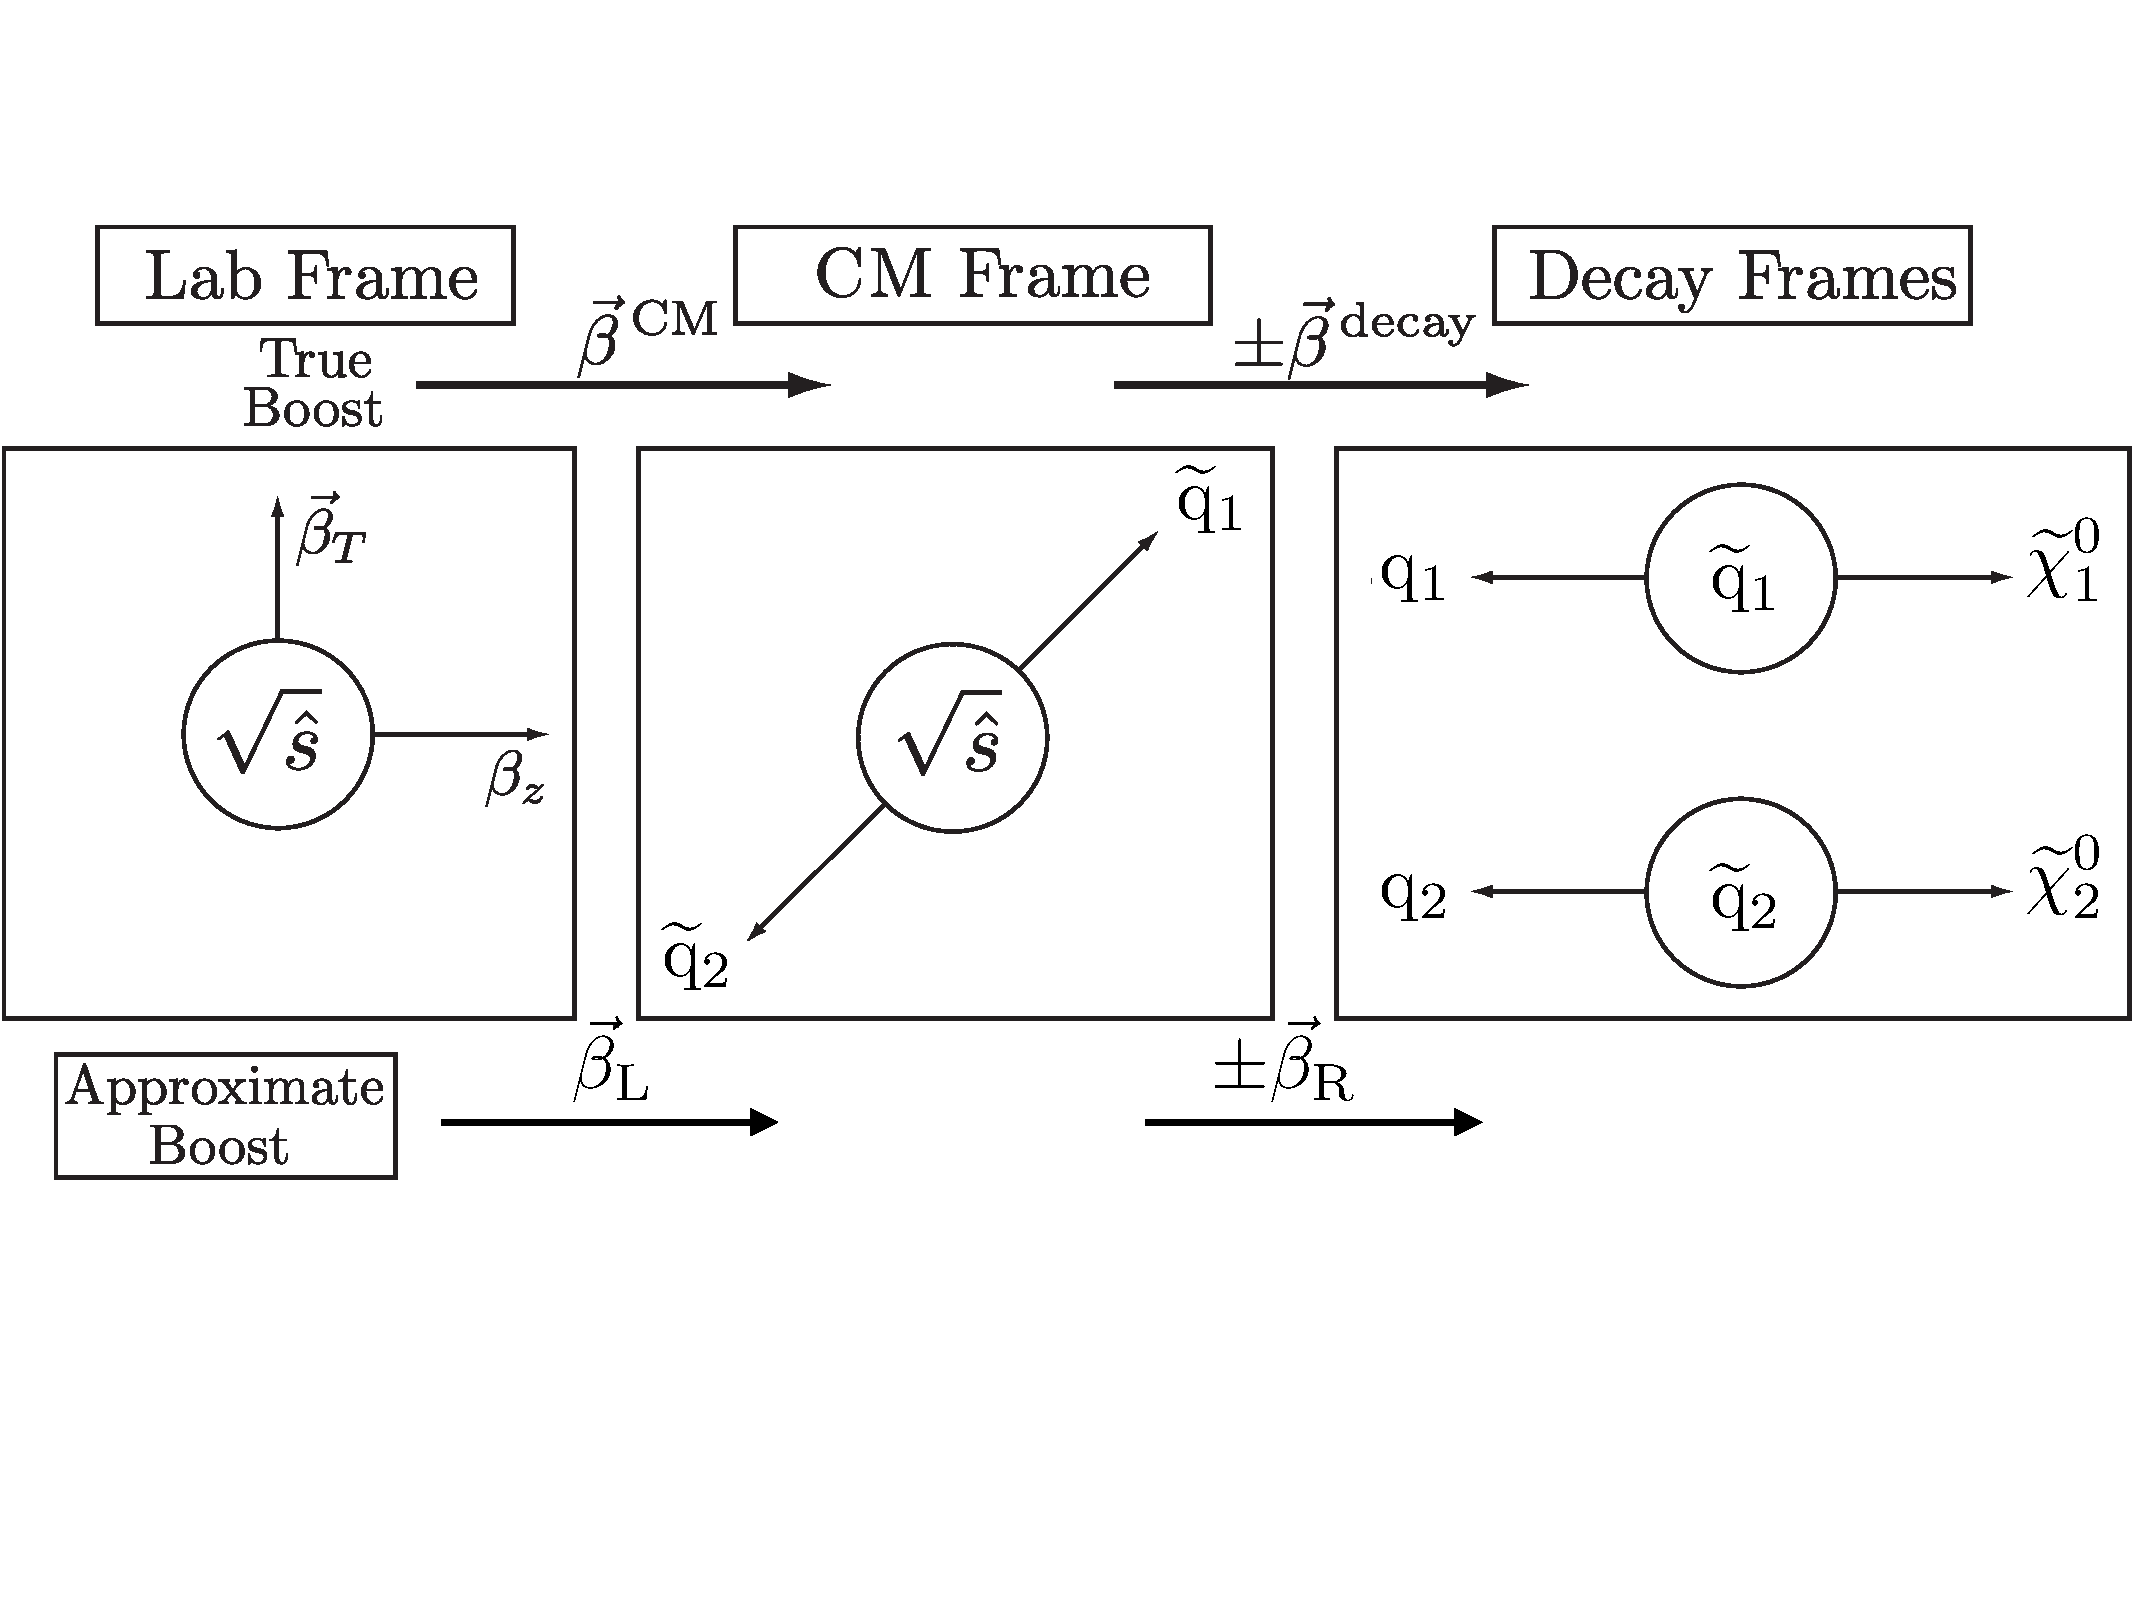
\includegraphics[width=0.95\textwidth]{figs/theory/frames3.pdf}
\caption{Three types of rest frames relevant to LHC pair production
  and the boosts relating them.\label{fig:frames}}
\end{figure*}

The crux of the razor approach is constructing estimators for these
boosts using physically-motivated assumptions and minimizing or
maximizing certain quantities-of-interest to determine any
underconstrained degrees of freedom. 

Following this blueprint, we first construct an
estimator of $\vec\beta^{\mathrm{CM}}$ called $\vec\beta_{\mathrm{L}}$~\cite{rogan,SuperRazor},
\begin{equation}
\vec\beta_{\mathrm{L}} = \beta_{\mathrm{L}}\hat{z} =
\frac{p^{\Pq_1}_z+ p^{\Pq_2}_z}{E^{\Pq_1}+ E^{\Pq_2}}\hat{z}~.
\end{equation}
This boost can be thought of as ``zeroing'' out the $z$-component of
the total visible momentum $P^{\,\mathrm{visible}}_z=0$, which
approximates the fact that in the true CM frame, we would have
\begin{equation}
P^{\mathrm{visible}}_z + P^{\mathrm{invisible}}_z = 0~.
\end{equation}
After performing this boost, we can compute the longitudinally
boost-invariant mass,
\begin{equation}
(\MR)^2 =(E_{\Pq_1}^{\prime}+ E_{\Pq_2}^{\prime})^2 = (E_{\Pq_1}+ E_{\Pq_2})^2 - (p^{\Pq_1}_z+ p^{\Pq_2}_z)^2~,
\end{equation}
where
\begin{equation}
E_{\Pq_i}^{\prime} = \gamma_{\mathrm L}E_{\Pq_i} - \vec\beta_{\mathrm
  L}\cdot \vec p^{\,\Pq_i} ~.
\end{equation}

To complete the ``razor picture'' of approximate rest frames, we can
construct another boost $\vec\beta_{\mathrm R}$, an estimator of $\vec\beta^{\mathrm{decay}}$, intended to be
applied asymmetrically to $\Pq_1$ and
$\Pq_2$~\cite{rogan,SuperRazor}. We know that after applying this
boost, the particles $\Pq_1$ and $\Pq_2$ must have the same energy in
their respective decay frames. This symmetry condition imposes a
constraint on $\vec\beta_{\mathrm R}$
\begin{align}
E_{\Pq_1}^{\prime\prime} = E_{\Pq_2}^{\prime\prime} &\Rightarrow \gamma_{\mathrm R}E_{\Pq_1}^{\prime} - \vec\beta_{\mathrm
  R}\cdot \vec p^{\,\Pq_1\prime} =  \gamma_{\mathrm R}E_{\Pq_2}^{\prime} + \vec\beta_{\mathrm
  R}\cdot \vec p^{\,\Pq_2\prime} \\
&\Rightarrow \vec\beta_R\cdot(\vec p^{\,\Pq_1\prime} + \vec
  p^{\,\Pq_2\prime}) = E^{\Pq_1\prime}- E^{\Pq_2\prime}
\end{align}
%where
%\begin{align}
%E_{\Pq_1}^{\prime\prime} &= \gamma_{\mathrm R}E_{\Pq_1}^{\prime} - \vec\beta_{\mathrm R}\cdot \vec p^{\,\Pq_1\prime} \\
%E_{\Pq_2}^{\prime\prime} &= \gamma_{\mathrm R}E_{\Pq_2}^{\prime} + \vec\beta_{\mathrm R}\cdot \vec p^{\,\Pq_2\prime} ~.
%\end{align}
Using symmetry, and the extremal condition $\partial (
E_{\Pq_1}^{\prime\prime} + E_{\Pq_2}^{\prime\prime} )/ \partial
\vec\beta_R = 0$, we arrive at the boost
\begin{equation}
\vec\beta_{\mathrm{R}} = 
\frac{\vec p^{\Pq_1\prime} - \vec p^{\Pq_2\prime}}{E^{\Pq_1\prime}+ E^{\Pq_2\prime}}~.
\end{equation}
After this boost, we see $\MR$ can be expressed as 
\begin{equation}
\MR =2\gamma_{\mathrm R} E_{\Pq_1}^{\prime\prime} = 2\gamma_{\mathrm R} E_{\Pq_2}^{\prime\prime} ~.
\end{equation}
We expect that the distribution of \MR for signal events will have a
peak near $M_{\Delta}$ if our assumptions that the pair production is near threshold
and $p^{\Pq_1}_z \approx -p^{\Pq_2}_z$ are correct in an average
statistical sense. Background events, in general, will not have
any special feature near $M_{\Delta}$. For example, events consisting
only of visible particles and $\ptvecmiss$ from mismeasurement, such
as QCD dijet production, would be expected to have a steeply falling \MR distribution
related to the distribution of the CM energy $\sqrt{\hat{s}}$.

We can also define a second mass variable that inherits knowledge of
the mass splitting $M_{\Delta}$, using the visible and invisible transverse
momentum in the event. Note that this information was not used in the
definition of \MR. Motivated by the fact that backgrounds with no
invisible particles must have $\Pq_1$ and $\Pq_2$ back-to-back (a fact
that mismeasurement dos not tend to greatly change), we define a
transverse mass in terms of the visible transverse momenta and the
missing transverse energy:
\begin{equation}
\MRT = \sqrt{ \frac{\ETm(\pt^{\Pq_1}+\pt^{\Pq_2}) -
\ptvecmiss \cdot
 (\ptvec^{\,\Pq_1}+\ptvec^{\,\Pq_2}) }{2}},
\end{equation}
Assuming pair production at threshold, $\MRT \leq M_{\Delta}$ for
signal events. The razor dimensionless ratio is defined as
\begin{equation}
\R \equiv \frac{\MRT}{\MR}.
\end{equation} 
we expect $\Rtwo\sim 1/4$ for signal events , while for background
without real missing transverse energy, we expect $\Rtwo \sim 0$. Note
that by construction, $\MRT \leq \MR$ and thus $R^2\leq 1$ if the
missing transverse momentum perfectly balances the visible transverse momentum
(as is necessary in the dijet case).

To generalize this approach to the case with an arbitrary number of visible
final state particles, we treat each event
as a dijet-like event by clustering particles into two pseudojets
called \emph{megajets}. 

Then, we may compute, \MR and $\MRT$, defined as
\begin{align}
 \label{eq:MRstar}
 \MR &\equiv
 \sqrt{
(\abs{\vec{p}^{j_{1}}}+\abs{\vec{p}^{j_{2}}})^2 -({p}^{j_1}_z+{p}^{j_2}_z)^2},\\
\MRT &\equiv \sqrt{ \frac{\ETm(\pt^{j_1}+\pt^{j_2}) -
\ptvecmiss \cdot
 (\ptvec^{\,j_1}+\ptvec^{\,j_2}) }{2}},
\end{align}
where $\vec{p}_{j_i}$, $\ptvec^{\,j_i}$, and
$p^{j_i}_z$ are the momentum of the $i$th megajet, its
transverse component with respect to the beam axis, and its
longitudinal component, respectively, with $\ETm$ the magnitude of $\ptvecmiss$. While
$\MRT$ quantifies the transverse momentum imbalance,
$\MR$ estimates the mass scale of new-physics particle
production in the event. 


\begin{figure*}[thb!]
\centering
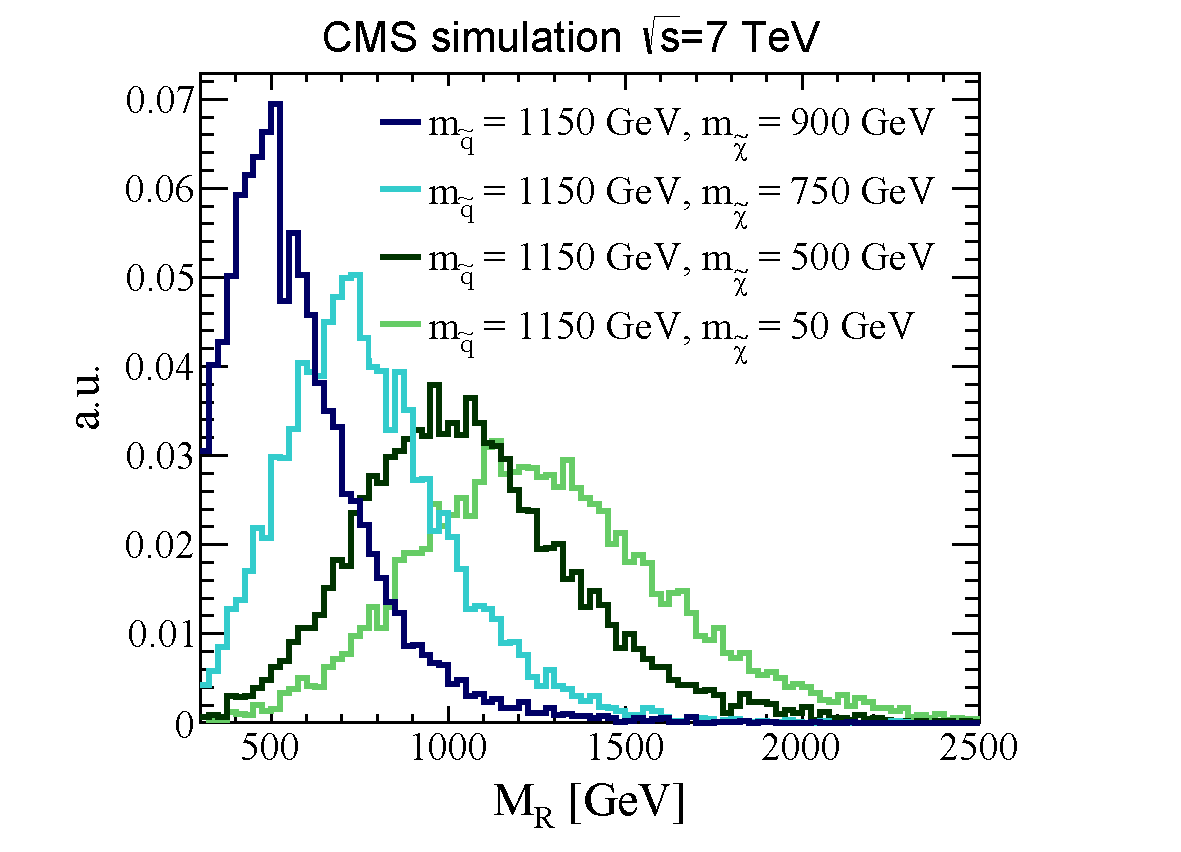
\includegraphics[width=0.49\textwidth]{figs/theory/MR_T2_pheno.pdf}
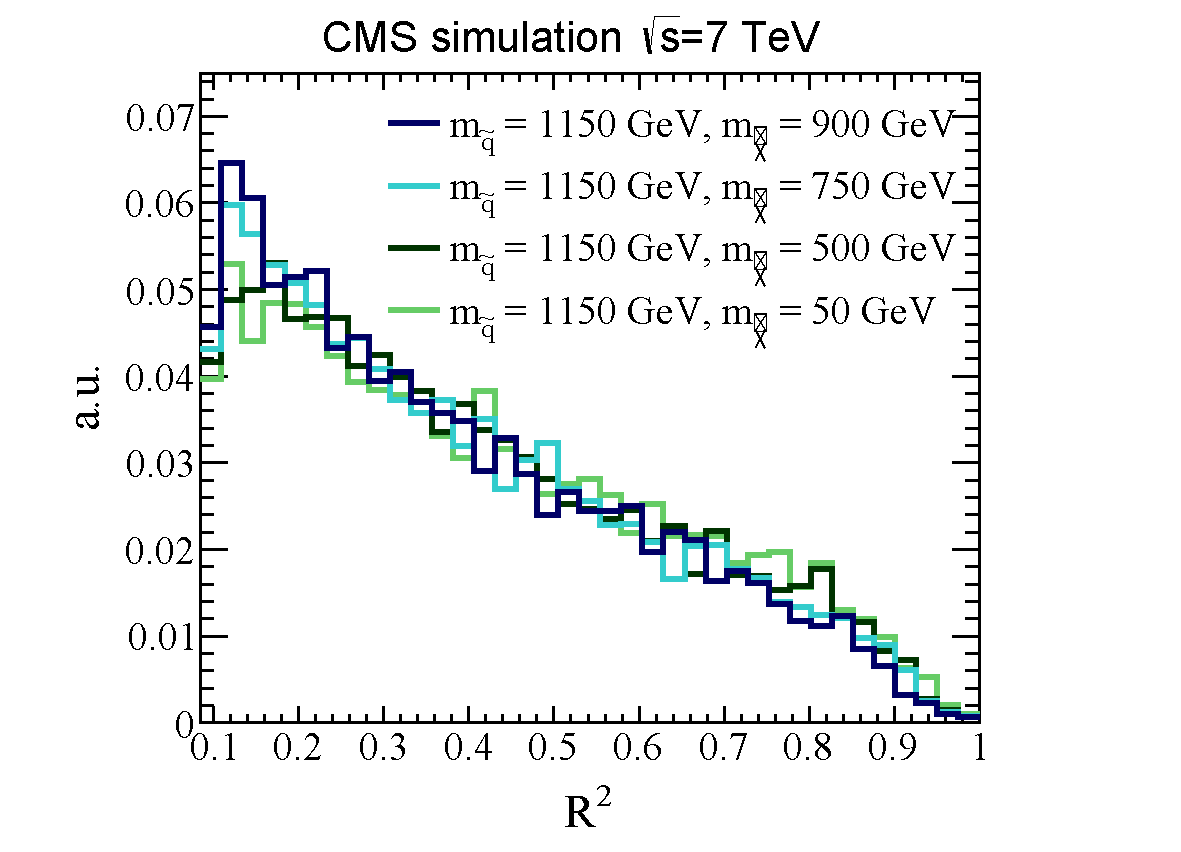
\includegraphics[width=0.49\textwidth]{figs/theory/RSQ_T2_pheno.pdf}\\
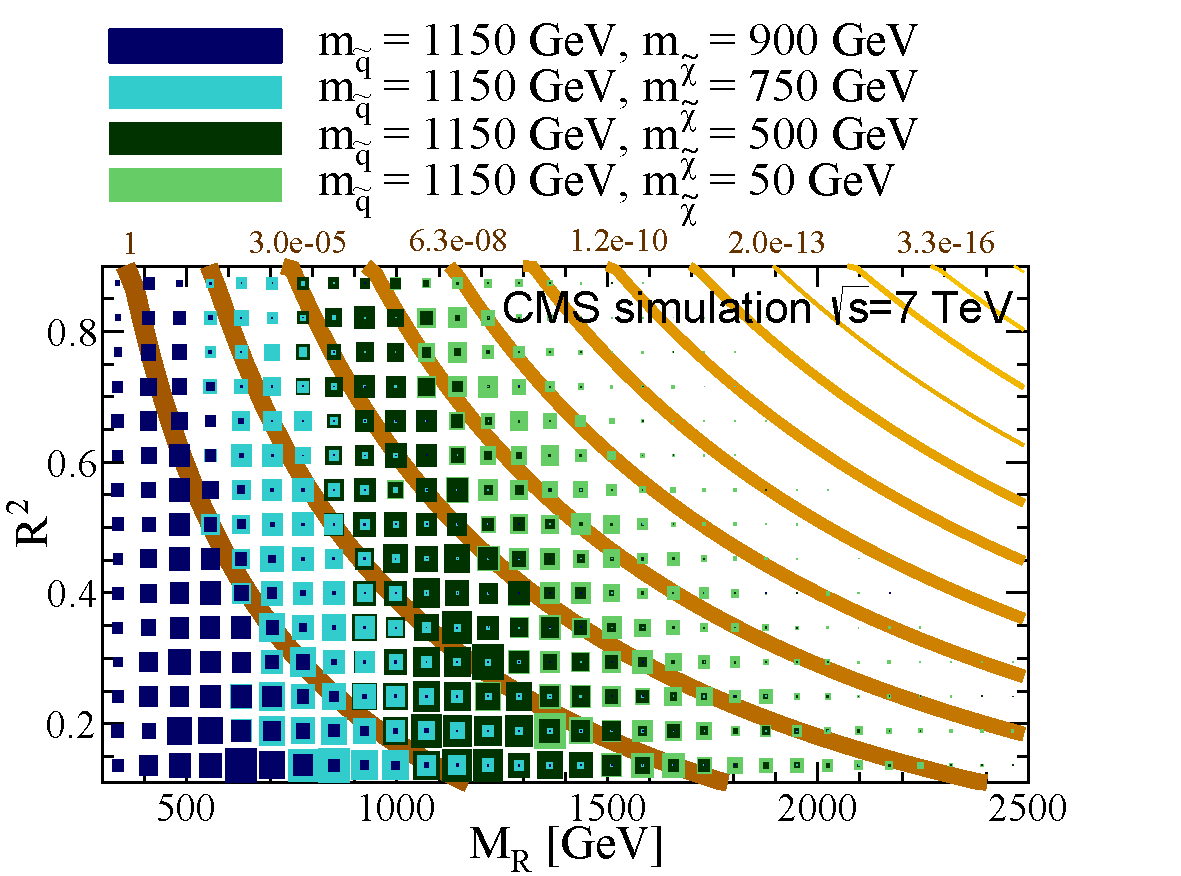
\includegraphics[width=0.49\textwidth]{figs/theory/MR_T2_R2_pheno.pdf}
\caption{Distribution of \Rtwo and \MR for different squark and LSP masses.\label{fig:T2RsqMR}}
\end{figure*}

\textbf{NEED TO EXPAND ON KINEMATICS A LOT}

